%
% File emnlp2019.tex
%
%% Based on the style files for ACL 2019, which were
%% Based on the style files for EMNLP 2018, which were
%% Based on the style files for ACL 2018, which were
%% Based on the style files for ACL-2015, with some improvements
%%  taken from the NAACL-2016 style
%% Based on the style files for ACL-2014, which were, in turn,
%% based on ACL-2013, ACL-2012, ACL-2011, ACL-2010, ACL-IJCNLP-2009,
%% EACL-2009, IJCNLP-2008...
%% Based on the style files for EACL 2006 by
%%e.agirre@ehu.es or Sergi.Balari@uab.es
%% and that of ACL 08 by Joakim Nivre and Noah Smith

\documentclass[11pt,a4paper]{article}
\usepackage[hyperref]{emnlp-ijcnlp-2019}
\usepackage{hyperref}
\usepackage{times}
\usepackage{latexsym}
\usepackage{graphicx}

%\usepackage{url}

\aclfinalcopy % Uncomment this line for the final submission

%\setlength\titlebox{5cm}
% You can expand the titlebox if you need extra space
% to show all the authors. Please do not make the titlebox
% smaller than 5cm (the original size); we will check this
% in the camera-ready version and ask you to change it back.

\newcommand\BibTeX{B{\sc ib}\TeX}
\newcommand\confname{EMNLP-IJCNLP 2019}
\newcommand\conforg{SIGDAT}

\title{reproducing ``ner and pos when nothing is capitalized"}

\author{Andreas Kuster \\
    {\tt kustera@student.ethz} \\\And
    Jakub Filipek \\
    {\tt balbok@uw} \\\And
    Viswa Virinchi Muppirala \\
    {\tt virinchi@uw}}
\date{}

\makeatletter
\def\endthebibliography{%
	\def\@noitemerr{\@latex@warning{Empty `thebibliography' environment}}%
	\endlist
}
\makeatother

\begin{document}
\maketitle
\begin{abstract}
    Capitalization is an important feature in many NLP tasks such as Named Entity Recognition (NER) or Part of Speech Tagging (POS). We are trying to reproduce results of paper which shows how to mitigate a significant performance drop when casing is mismatched between training and testing data. In particular we show that mixing cased and uncased dataset provides the best performance, matching the claims of the original paper. We also show that we got slightly lower performance in almost all experiments we have tried to reproduce, suggesting, that the orginal paper did not fully disclose all of the experimental setup.
\end{abstract}

\section{Introduction}
Previous works have shown that there is a significant performance drop when applying models trained on cased data to uncased data and vice-versa \cite{wang-etal-2006-capitalizing}. Since capitalization is not always available due to real world constraints, there have been some methods trying to use casing prediction (called \textit{truecasing}) to battle this trade-off.

The work we reproduce tries to battle this issue in two popular NLP tasks by mixing both cased and uncased datasets.

\section{Contributions}
This paper effectively shows how well work from \cite{ner-and-pos-original} can be reproducede and how well it applies to a few other settings.\\
Original paper does show how casing issue in NLP can be effectively solved through a method which requires close to none overhead in terms of development time, and no additional overhead in runtime, especially when compared to methods such as truecasing.\\
It also serves as a reproducing work to show that truecasing can be reproduced. We show that while truecasing experiment can be reproduced on the same experiment, but claims on applicability to other datasets fail to reproduce.

\subsection{Hypotheses from original paper}
\label{sec:original_hypotheses}
Original paper proposes following hypotheses:
\begin{itemize}
    \item Truecasing fits strongly to data it is presented leading to performance drops on different datasets.
    \item Mixing cased and uncased data provides the best performance in NER task on CoNLL 2003 dataset.
    \item Such techinque generalizes well on noisy datasets such as Twitter data.
    \item Mixing cased and uncased data provides the best performance in POS task on Penn Treebank dataset.
\end{itemize}

\subsection{Hypotheses addressed in this work}
\label{sec:current_hypotheses}
In addition to hypotheses tested in Section~\ref{sec:original_hypotheses} we also tested:
\begin{itemize}
    \item POS:
    \begin{itemize}
        \item Mixing both cased and uncased data leads to the best performance regardless of word \textbf{embedding} used.
        \item Mixing both cased and uncased data leads to the best performance regardless of word \textbf{dataset} used.
        \item Using ELMo model with CRF layer in POS task to outperform the one without, regardless of data casing technique. This is based on \cite{BiLSTM-CRF}.
    \end{itemize}
\end{itemize}


\subsection{Experiments}
We conducted two main experiments from the paper, and tried to confirm the reproducibility claim that the original paper made.

Truecasing is a task where given all lowercase sentences we have to predict correct casing. Here we trained a simple Bidirectional LSTM with a logical layer on top, as described in both \cite{ner-and-pos-original} and \cite{susanto-etal-2016-learning}. Since the former paper, does a great job of mentioning hyper-parameters used in the network, the hyperparameter search is not required.

Part of Speech tagging is a task in which given a sentence we have to predict part of speech for each word. It is our the most in depth experiment, which lead a lot of additional hypotheses which got tested. Firstly, we had to find optimal hyper-parameter setting. The search was not too large, since a few of the parameters (such as number of layers) were known, but it still took a significant amount of time. After finding such setting we compared its results with ones reported the original paper. Then we investigated whether claims from this paper are applicable to other datasets and encodings. Lastly, we looked at the CRF layer, and what its impact on performance on the whole model is.

Named Entity Recognition is a task in which given a sentence we have to predict which parts of it describe some entity. It had the most sophisticated model out of all the experiments we tried reproducing. Fortunately we did not have to do a hyperparameter search since \cite{ner-and-pos-original} and \cite{ma-hovy-2016-end} described model rather well for NER task.

\section{Code}
There are no public repos which do mention the project in their \textit{READMEs}.

However, in case of truecasing, primary author of \cite{ner-and-pos-original} has two repositories: \href{https://github.com/mayhewsw/truecaser}{truecaser} and \href{https://github.com/mayhewsw/pytorch-truecaser}{python-truecaser}. The former one refers to the original implementation from \cite{susanto-etal-2016-learning}, while the python one is a port to python. The (probably) primary author of \cite{susanto-etal-2016-learning} also has a \href{https://github.com/raymondhs/char-rnn-truecase}{github repository} possibly related to truecaser we are trying to reproduce. However, to validate results and test ease of application we decided to not use either of these resources and focus on custom implementation. This also removes dependence on Andrej Karpathy's \href{https://github.com/karpathy/char-rnn}{char-rnn} all of the above mentioned repositories are forks of.

We were not able to find publicly available code for either NER or POS parts of the original paper.

Hence we needed to reimplement the code from scratch. All our work is in \href{https://github.com/andreaskuster/uw-nlp}{public github repository}. We tried to make all results as easily accessible as possible, which means that there is significant overlap between this report and the \textit{README} on that repository.

Truecasing and NER were implemented using PyTorch \cite{pytorch}, while POS was implemented in Keras \cite{keras}, on top of TensorFlow \cite{tensorflow2015-whitepaper}.

\section{Experimental setup and results}

\subsection{Datasets}
\label{sec:datasets}
Datasets were a common resource about all three parts of experiments. Hence we will describe them separate here, and for each experiment specify which exact dataset was used:
\begin{itemize}
    \item CoNLL2003 - From \cite{conll2003}. Not publicly available. Shared as part of class.
    \item Peen Tree Bank (PTB) - From \cite{penn-treebank}. Not publicly available. Shared as part of class. We used a loader from \href{https://www.nltk.org/}{nltk} (after appending nonpublic data to it). In particular:
        \begin{itemize}
            \item Sections 0-18 are used for training
            \item Sections 19-21 are used for development, i.e. choosing hyperparameters
            \item Sections 22-24 are used for test, i.e. reporting accuracy
        \end{itemize}
    \item Twitter - From \cite{twitter-dataset}. Specifically we found \href{https://github.com/GateNLP/broad_twitter_corpus}{authors github repository} with data available.
    \item Wikipedia - From \href{https://github.com/raymondhs/char-rnn-truecase/tree/master/data/wiki}{github repository}, which we suspect is authored by primary author of \cite{susanto-etal-2016-learning}. This data was used for truecasing experiment.
\end{itemize}

Additionally, in case of NER and POS each of these datasets occurs in 5 different experimental flavors:
\begin{itemize}
    \item Cased (C) - Standard dataset, as downloaded.
    \item Uncased (U) - Uncased dataset. It's a standard dataset, with an additional step of converting everything to lowercase.
    \item Cased + Uncased (C + U) - Combination of both cased and uncased flavors. Hence it is twice the size of either cased or uncased.
    \item Half Mixed (C + U 50) - Combination of cased and uncased flavors. However, only 50\% of data is lowercase, and remaining half is as-is.
    \item Truecase Test (TT) - Truecased Test dataset. Training data is the same as cased one. Test is converted to uncased version, and then a trucaser is run on it.
    \item Truecase All (TA) - Truecased Train and Test dataset. The transformation described for test in TT is applied to both train and test.
\end{itemize}

\subsection{Padding}
To remove repetition in description of experiments we also want to discuss padding and how results should be understood.

All experiments described below used padding to the maximum sentence size for training. However, for results on both validation (development) and test such padding was either removed or ignored, and hence it is not affecting the results reported in this paper.

\subsection{Truecasing}
\label{sec:exp-truecase}

    \subsubsection{Model description}
    We used the exact same model as described in \cite{susanto-etal-2016-learning}, a 2 layer, bidirectional LSTM. Since encoding was not specified, nor any character level encoding was mentioned in class we used a PyTorch \cite{pytorch} Encoder layer, which learned weights from bag-of-words to a feature-sized word representation. Note that in this model size of word embeddings is equal to hidden state size (both 300 dimensional). Then on top of these two layer a binary linear layer was applied.

    Hence output of this model is 2 dimensional, one specifying that character should be upper cased (true), other that character should be left as is.

    Implementation of this model took 2 hours, mostly due to transposes required by LSTM layers in PyTorch framework. It also helped that assignment 2 required us to implement LSTM model, and we could reuse parts of it.

    \subsubsection{Hyperparameters}
    We used a 2 layer, bidirectional LSTM with hidden size of 300. On top of that a linear layer, with 2 classes was applied, resulting in binary output. We used Adam \cite{adam} optimizer with default settings (learning rate of 0.001, betas of 0.9 and 0.999), and batch size of 100, as suggested in the \cite{susanto-etal-2016-learning}. Since these were the hyperparameters specified, we did not perform hyperparameter search.

    We also used an Out-Of-Vocabulary (OOV) rate of 0.5\%. Due to initial mistake we first defined out-of-vocabulary rate in following manner. When each token was drawn it had a 0.5\% chance to be masked with OOV token.

    However, after clarification from TA we switched OOV to be done at the initialization of tokens. In particular sorted tokens in order of increasing occurrence, and masked all least occurring tokens (such that their sum contained at least 0.5\% of total amount of tokens) with OOV token. This skewed our OOV distribution towards uncommon tokens. This is a desired behavior, due to the fact that the differences between datasets will be in these rare-occurring tokens.

    For wikipedia dataset, with first approach we got a dictionary of size 64, and with second approach it was 41.

    \subsubsection{Results}
    We trained these models for 30 epochs, with crossentropy loss. We recorded both training and validation loss for both, and chose the models with lowest validation loss for each of OOV settings. In both cases, such point was reached after around 7-8 epochs.

    The performance of the model matched one claimed both by original paper, and original truecasing paper on Wikipedia dataset. However, there was a significant mismatch in performance on other datasets provided in the original paper. This can be seen in Table \ref{tab:truecase-result}. A drop-off between datasets is expected, because as explained in original paper, various sources will use various casing schemes specific to the domain.
    \begin{table}[h]
        \centering
        \begin{tabular}{|l|c|c|}
            \hline
            Dataset & Initial OOV & Proper OOV \\
            \hline
            Wikipedia & 92.65 & 92.71\\
            \hline
            \hline
            CoNLL Train & 66.03 & 65.32 \\
            \hline
            CoNLL Test & 63.49 & 63.28 \\
            \hline
            PTB 01-18 & 78.53 & 78.73 \\
            \hline
            PTB 22-24 & 78.47 & 78.69 \\
            \hline
        \end{tabular}
        \caption{F1 scores of best performing model (chosen on validation set of Wikipedia dataset) for various datasets. Initial OOV stands for at-the-read techinque of creating OOV tokens, while proper is the former one of two described above.}
        \label{tab:truecase-result}
    \end{table}
    For reference Table \ref{tab:trucase-original-result} contains results from investigated papers. We can see that there is not a high difference in performance between results for Wikipedia dataset, but there is a 10\% difference in both CoNLL and PTB between our results and original ones. The possible reason for it might be the fact that original paper used fork of, before mentioned, \href{https://github.com/karpathy/char-rnn}{char-rnn}. We looked at it, searching for differences between our intuition and actual implementation, but could not find any.
    \begin{table}[h]
        \centering
        \begin{tabular}{|l|c|}
            \hline
            Dataset & Original \\
            \hline
            Wikipedia (Susanto) & 93.19 \\
            \hline
            Wikipedia & 93.01 \\
            \hline
            \hline
            CoNLL Train & 78.85 \\
            \hline
            CoNLL Test & 77.35 \\
            \hline
            PTB 01-18 & 86.91 \\
            \hline
            PTB 22-24 & 86.22 \\
            \hline
        \end{tabular}
        \caption{F1 scores from reference papers. All entries but ``Wikipedia (Susanto)" are from \cite{ner-and-pos-original}.}
        \label{tab:trucase-original-result}
    \end{table}
    This leaves us in conclusion that, in terms of performance, this experiment can be only partially reproduced, and it is possible that additional techniques (such as dropout, etc.) were applied during training of the model. However, in terms of between-datasets trends the paper describes, we have confirmed them, and \textbf{were able to (partially) reproduce the first hypothesis of the paper}.

\subsection{Part of Speech Tagging}
\label{sec:exp-pos}

    \subsubsection{Model description}
    Model for POS task is not well described in the original paper, and rather references other papers for implementation details \cite{ma-hovy-2016-end}. This left us with only a rough sketch of a model, and a hyperparameter search for most of variables.

    Model used here is a single BiLSTM layer, followed by a Time Distributed Dense layer, followed by an output CRF layer. We used ELMo as the encoding for the input to BiLSTM layer.

    \subsubsection{Hyperparameters}
    \label{sec:exp-pos-hyper}
    As mentioned before, the task required a hyperparameter search. It was performed on standard (Cased) version of PTB dataset. Due to time constraints we opted for grid search with following settings:
    \begin{table}[h]
        \centering
        \begin{tabular}{|l|l|l|}
            \hline
            Hyperparameter & Values & Best \\
            \hline
            LSTM Hidden Units & $2^{\{0, 1, 2, 3, 5, 7, 9\}}$ & 512 \\
            \hline
            LSTM Drop. & 0.0, 0.2, 0.4 & 0.0 \\
            \hline
            LSTM Recurr. Drop. & 0.0, 0.2, 0.4 & 0.0 \\
            \hline
            learning rate & 0.1, 0.001 & 0.001 \\
            \hline
        \end{tabular}
        \caption{Hyperparamter Search for POS experiment. Values investigated are in the middle column, while optimal combination of hyperparameters is in the right one.}
        \label{tab:pos-hypersearch}
    \end{table}

    One of the surprises of optimal setting is that both of dropout's are zero. However, as seen on Fig. \ref{fig:pos-hyperdrop}, we can see that all settings converge to roughly the same performance on validation set, with $0.0$ having the fastest convergence.

    \begin{figure}[h]
        \centering
    	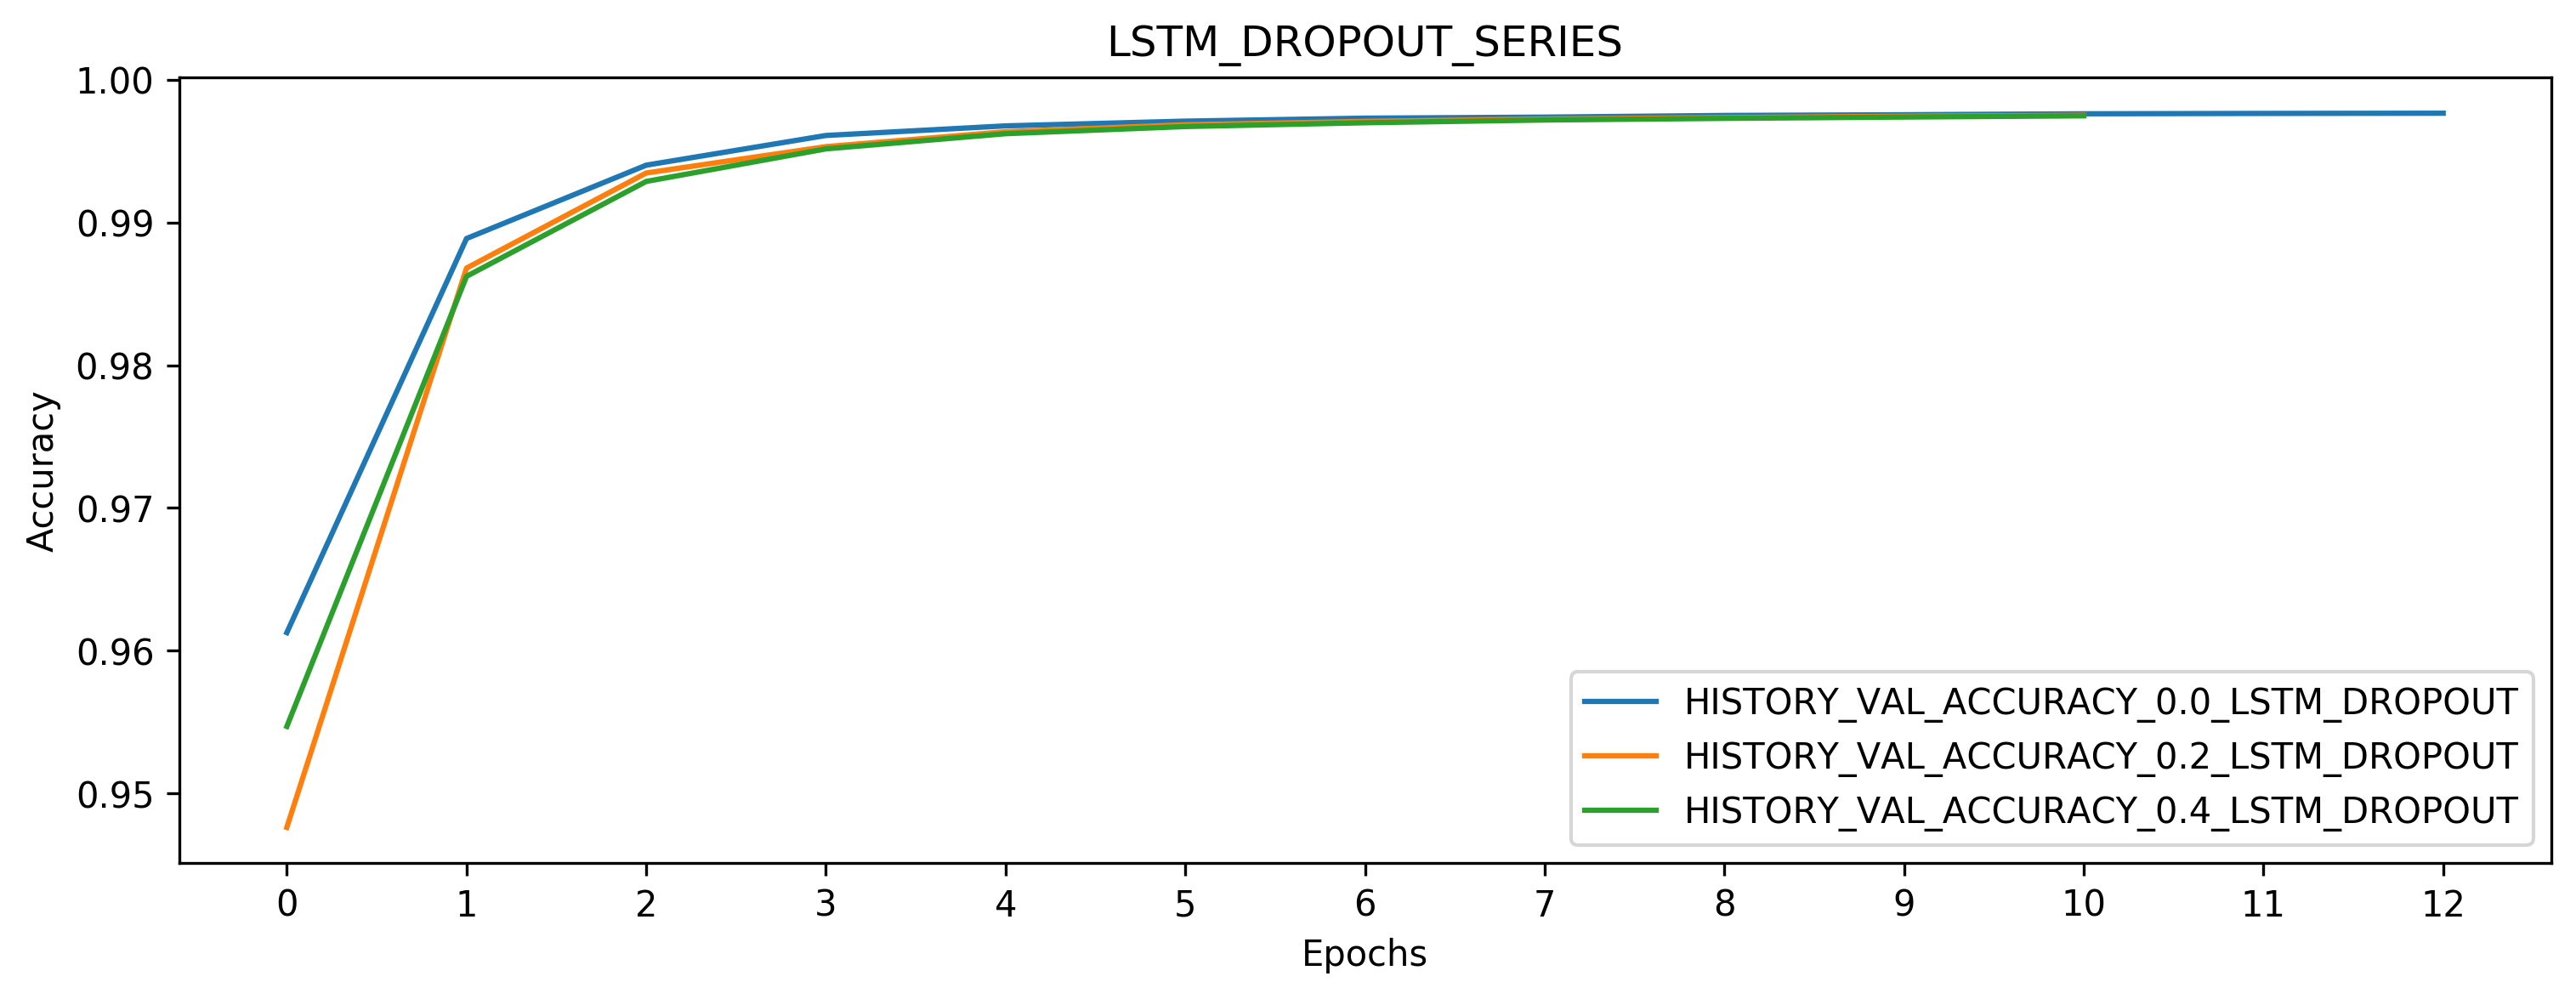
\includegraphics[scale=0.3]{pos_hypersearch_drop.png}
        \caption{Performance of various settings for different dropout values in LSTM layer.}
        \label{fig:pos-hyperdrop}
    \end{figure}

    Sizes of Time Distributed Dense layer, and CRF layer are the same, and equal to number of classes given dataset. Additionally size of ELMo encoding (and hence size of input to BiLSTM layer) is 1024.

    Due to time constraints we also used early stopping. Training was stopped either after 40 epochs or if validation accuracy improvement was smaller than 0.001 over 4 epochs.

    \subsubsection{Results}
    We tested the optimal model on 5 different setups, as described in list of flavors in Sec. \ref{sec:datasets}. The dataset used in this case was PTB, with splits as described before.

    \begin{table}[h]
        \centering
        \begin{tabular}{|l|c|c|c|}
            \hline
            Exp. & Test (C) & Test (U) & Avg \\
            \hline
            C        & 97.30 & 88.29 & 92.78 \\
            U        & 96.51 & 96.51 & 96.51 \\
            C + U    & 97.51 & 96.59 & \textbf{97.05} \\
            C + U 50 & 97.12 & 96.19 & \textbf{96.66} \\
            TT       & 95.04 & 95.04 & 95.04 \\
            TA       & 96.61 & 96.61 & 96.61 \\
            \hline
        \end{tabular}
        \caption{Accuracies for the POS task, in our setup. Averages of two best performing flavors are emboldened for readability.}
        \label{tab:pos-results-our}
    \end{table}

    \begin{table}[h]
        \centering
        \begin{tabular}{|l|c|c|}
            \hline
            Exp. & Our & Original \\
            \hline
            C        & 92.78 & 93.26 \\
            U        & 96.51 & 97.45 \\
            C + U    & \textbf{97.05} & \textbf{97.57} \\
            C + U 50 & \textbf{96.66} & \textbf{97.61} \\
            TT       & 95.04 & 95.21 \\
            TA       & 96.61 & 97.38 \\
            \hline
        \end{tabular}
        \caption{Comparison of average accuracies for the POS task. Results on the left are using our code, while ones of the left are reported in the original paper. For both sources 2 best results are emboldened.}
        \label{tab:pos-results-comp}
    \end{table}

    We can see that we agree with the hypothesis that mixing cased and uncased provides the best performance on the Penn Tree Bank as can be seen in Table \ref{tab:pos-results-our}. This confirms the hypothesis.

    However, as in case of Truecasing, we conclude that in terms of absolute performence we did get different results as reference paper. This can be seen in Table \ref{tab:pos-results-comp}, where there is about 1\% difference in accuracy between our implementation and the original one. In addition to this the gain due to mixing cased and uncased data is sometimes smaller than the difference between implementations, such as in case of Uncased flavor, where reference has higher accuracy than our C + U flavor.

    Overall, \textbf{we confirm the hypothesis}, but with a grain of salt due to lack of transparency in implementation in the original paper.


\subsection{Named Entity Recognition}
\label{sec:exp-ner}

    \subsubsection{Model description}
    \textcolor{green}{See syllabus. If you had to implement the model, record how long each part took.}

    \subsubsection{Hyperparameters}
    \textcolor{green}{See syllabus. Describe what you can.}

    \subsubsection{Results}
    \textcolor{green}{Each experiment should have: a clear explanation of how it was run, the high-level takeaway, a pointer to the hypothesis it supports, and it should say whether it reproduces the experiments in the original paper or not.}

\section{Experiments beyond the original paper}

    \subsection{Datasets}
    In addition to the datasets used in original paper, we additionally used:
    \begin{itemize}
        \item Brown - From \href{http://korpus.uib.no/icame/brown/bcm.html}{Brown University}. We used a loader from \href{https://www.nltk.org/}{nltk}.
        \item CoNLL2000 - From \cite{conll2000}. We used a loader from \href{https://www.nltk.org/}{nltk}.
        \item PTB Reduced (PTB R) - Same as Penn Tree Bank described in Section \ref{sec:datasets}, but:
        \begin{itemize}
            \item Train consists of sections 0-4
            \item Validation consists of sections 5-6
            \item Test consists of sections 7-8
        \end{itemize}
    \end{itemize}

    \subsection{Part of Speech Tagging}
    The aim of the additional experiments is to find out if the hypothesis from the paper is more generally applicable. We run the same experiments on LSTM models with different word embeddings, with or without the CRF layer, and on different datasets.

    \subsubsection{Hyperparameters}
    Due to results in Section \ref{sec:exp-pos-hyper} the same model was used as in the original experiment.

    One important note for encodings is that they change number of inputs to BiLSTM layer, thus slightly modifying its size. In particular both GloVe and word2vec have size of 300, which is much smaller than 1024 in ELMo.

    \subsubsection{Results}
    Since there were 3 experiments roughly separate experiments let us present them separately.

    \begin{table}[h]
        \centering
        \begin{tabular}{|l|c|c|c|}
            \hline
            Exp.     & word2vec       & GloVe          & ELMo \\
            \hline
            C        & 83.71          & 91.01          & 92.78 \\
            U        & 80.97          & 94.67          & 96.51 \\
            C + U    & \textbf{86.15} & \textbf{96.36} & \textbf{97.05} \\
            C + U 50 & 85.01          & \textbf{95.35} & \textbf{96.66} \\
            TT       & 85.74          & 93.82          & 95.04 \\
            TA       & \textbf{86.64} & 95.20          & 96.61 \\
            \hline
        \end{tabular}
        \caption{Average accuracies for different encodings. Note that ELMo encodings are the exact copy of results from \ref{tab:pos-results-our}. Similarly to other tables 2 best scores are emboldened for readability.}
        \label{tab:epos-encodings}
    \end{table}

    Table \ref{tab:epos-encodings} shows results for various encodings. We see that we consistently mixed dataset appears to be in the top 2 results. We can also see that encoding has a strong effect on absolute performance of the model, especially in case of word2vec which has a 10\% drop in accuracy relative to GloVe and ELMo. This is an expected behavior as ELMo is known to outperform both word2vec and GloVe in many cases.

    There is an interesting notion that both of Truecasing flavors tend to perform better than Half Mixed one. However, due to significant drop in word2vec with respect to other encodings we believe that it rather an artifact of the encoding itself rather than a theme. Additionally, performance of all three scenarios is rather close further pointing to encoding specific problem.

    Overall, we believe that the first additional hypothesis is \textbf{supported by the above results}.

    \begin{table}[h]
        \centering
        \begin{tabular}{|l|c|c|c|}
            \hline
            Exp. & PTB R & Brown & CoNLL2000 \\
            \hline
            C        & 92.36          & 89.50          & 92.86\\
            U        & 95.48          & 92.91          & 96.83 \\
            C + U    & \textbf{96.22} & \textbf{96.47} & \textbf{99.23} \\
            C + U 50 & \textbf{95.71} & \textbf{93.92} & \textbf{97.16} \\
            TT       & 94.62          & 92.11          & 95.40 \\
            TA       & 95.35          & 92.62          & 96.79 \\
            \hline
        \end{tabular}
        \caption{Average accuracies for different datasets.}
        \label{tab:epos-results-datasets}
    \end{table}

    Table \ref{tab:epos-results-datasets} shows results for different dataset. Here results are clear, mixing cased and uncased datasets provides the best result regardless of a dataset. In fact for Brwon CoNLL2000 gaps between this technique and others is even larger than on the original PTB dataset. Hence, these results \textbf{strongly support our second additional hypothesis}.

    \begin{table}[h]
        \centering
        \begin{tabular}{|l|c|c|}
            \hline
            Exp. & No CRF & CRF \\
            \hline
            C        & 92.88 & 92.78 \\
            U        & 96.52 & 96.51 \\
            C + U    & 97.02 & 97.05 \\
            C + U 50 & 96.83 & 96.66 \\
            TT       & 94.78 & 95.04 \\
            TA       & 96.56 & 96.61 \\
            \hline
        \end{tabular}
        \caption{Average accuracies for the original model with CRF and without CRF.}
        \label{tab:epos-results-crf}
    \end{table}

    Table \ref{tab:epos-results-crf} compares performance of the original model with or without the last layer. Considering that most of results are within a few hundredths between two models, with TT being 0.26\% away from the original implementation, we conclude that CRF can be eliminated from the model without major differences in performance. This is very beneficial on the implementation and runtime side, since CRF is a non-standard library, making model are complicated, and does not have multi-gpu support, causing it to run much longer. These results, \textbf{strongly support our third additional hypothesis}, and we recommend potential future users of BiLSTM to not include CRF layer (at least for POS task).

\section{Computational requirements}
Due to relative lack of overlap between three sections each of us used different computational resources:
\begin{itemize}
    \item Truecasing:
    \begin{itemize}
        \item GPU: NVIDIA RTX 2080 Super
        \item CPU: AMD Ryzen 7 3700x
        \item Runtime: 10h (Original Paper)
    \end{itemize}
    \item POS:
    \begin{itemize}
        \item GPU: 2x NVIDIA V100
        \item CPU: AMD EPYC 7501
        \item Runtime: 100h (Original Paper + Additional Experiments)
    \end{itemize}
    \item NER:
    \begin{itemize}
        \item GPU: NVIDIA GTX 1080
        \item CPU: Intel Core i7-6850K
        \item Runtime: 26h (Original Paper + Twitter Evaluation)
    \end{itemize}
\end{itemize}

This is required for every report. Include every item listed in the syllabus, plus any other relevant statistics (e.g. if you have multiple model sizes, report info for each).
Include the information listed in the syllabus, including the \textbf{total} number of GPU hours used for all experiments, and the number of GPU hours for \textbf{each} experiment.

\section{Discussion and recommendations}
Conclude the report, and summarize which hypotheses from the original paper were reproducible. Include suggestions for future researchers -- what was hard? What worked easily?

\bibliographystyle{acl_natbib}
\bibliography{emnlp-ijcnlp-2019}

\end{document}
